\documentclass[12pt,a4paper,utf8]{ctexart}
\usepackage{graphicx}
\usepackage{amsmath}
\usepackage{amssymb}
\usepackage{subfig}
\usepackage{cite}
\usepackage[ntheorem]{empheq}
\usepackage{enumitem}
\usepackage{fullpage}
\usepackage{cleveref}
\usepackage{cellspace}
\usepackage{listings}
\usepackage{color}
\usepackage{float}
\definecolor{gray}{rgb}{0.5,0.5,0.5}
\definecolor{dkgreen}{rgb}{.068,.578,.068}
\definecolor{dkpurple}{rgb}{.320,.064,.680}

% set Matlab styles
\lstset{
   language=Matlab,
   keywords={break,case,catch,continue,else,elseif,end,for,function,
      global,if,otherwise,persistent,return,switch,try,while},
   basicstyle=\ttfamily,
   keywordstyle=\color{blue}\bfseries,
   commentstyle=\color{dkgreen},
   stringstyle=\color{dkpurple},
   backgroundcolor=\color{white},
   tabsize=4,
   showspaces=false,
   showstringspaces=false,
   breaklines,%自动换行
   columns=flexible
}

\begin{document}
\CJKfamily{zhkai}	


\begin{center}
\textbf{作业一}\\
\textbf{敖旭扬 ~~~~~ PB18071477 ~~~~~ \today}\\
\end{center}
\textit{}
\vspace{\baselineskip}

\begin{enumerate}
\item[第一题] 

(a) 由节点多项式$\ell(x)=\prod\limits_{k = 0}^n\left(x-x_{k}\right)$得
\begin{equation}
   \ell'(x)=\sum_{i=1}^{n}\prod_{k \neq i}^{n}\left(x-x_{k}\right) 
\end{equation}
\begin{equation}
   \ell'(x_j)=\prod_{k \neq j}^{n}\left(x_{j}-x_{k}\right) 
\end{equation}
则有
\begin{equation}
   \frac{\ell(x)}{\ell'(x_j)(x-x_j)}=\frac{\prod_{k = 0}^n(x-x_{k})}{(x-x_j)\prod_{k \neq j}^{n}(x_{j}-x_{k})}
   =\frac{\prod_{k \neq j}^n(x-x_{k})}{\prod_{k \neq j}^{n}(x_{j}-x_{k})}=\ell_j(x)
\end{equation}
将上式代入原Lagrange插值多项式得
\begin{equation}
   p(x)=\sum_{j=0}^{n}f_{j}\ell_{j}(x)=\sum_{j=0}^{n}f_{j}\frac{\ell(x)}{\ell'(x_j)(x-x_j)}
   =\ell(x)\sum_{j=0}^{n}\frac{\lambda_j}{x-x_j}f_j
\end{equation}

(b)Lagrange插值多项式的误差为
\begin{equation}
   R(x)=f(x)-\ell(x)=\frac{f^{(n+1)}(\xi)}{(n+1)!}\prod_{k=0}^{n}(x-x_k)
\end{equation}
则由插值多项式的存在唯一性,对于函数
$\{f(x) = x^k , k=0 , l,\cdots\}, f^{(n+l)}(x) =0 \Rightarrow  R(x) = 0$
,关于节点$\{1,2,\cdots ,X_n\}$的Lagrange插值多项式就是其本身,即
\begin{equation}
   \ell(x)=\sum_{j=0}^{n}\ell_j(x)x_j^k=x^k,\qquad k=0,1,\cdots,n
\end{equation}
令$k=0$得
\begin{equation}
   \sum_{j=0}^{n}\ell_j(x)=1
\end{equation}
从而
\begin{equation}
   \sum_{j=0}^{n}\frac{\ell(x)}{\ell'(x_j)(x-x_j)}=\sum_{j=0}^{n}\ell_j(x)=1
\end{equation}
变形得
\begin{equation}
   \ell(x)=\frac{1}{\sum_{j=0}^{n}\frac{1}{\ell'(x_j)(x-x_j)}}=\frac{1}{\sum_{j=0}^{n}\frac{\lambda_j}{x-x_j}}
\end{equation}
将上式代入(a)中的\underline{重心插值公式的第一形式}得
\begin{equation}
   p(x)=\ell(x)\sum_{j=0}^{n}\frac{\lambda_j}{x-x_j}f_j
   =\sum_{j=0}^{n}\frac{\lambda_j f_j}{x-x_j} \bigg/ \sum_{j=0}^{n}\frac{\lambda_j}{x-x_j}
\end{equation}

(d)\textsc{Matlab}程序显示如下:
\begin{lstlisting}[frame=single]
clear, clc, clf
LW = 'linewidth'; lw = 2;

n = 5000;
x = zeros(n + 1, 1);
m = 10000;
xx = linspace(-1, 1, m)';
F = @(x)tanh(20 * sin(12 .* x)) + 0.02 * exp(3 .* x) .* sin(300 .* x);
f = F(x);
p1 = zeros(m, 1);
p2 = zeros(m, 1);
p = zeros(m, 1);
%% 基于Chebyshev点的第二形式的重心插值公式
for j = 1:n + 1
      x(j) = cos((j - 1) * pi / n);
end

p1 = 0.5 * (F(1) ./ (xx -1) + ((-1)^n) * F(-1) ./ (xx + 1));
p2 = 0.5 * (1 ./ (xx -1) + ((-1)^n) ./ (xx + 1));

for k = 2:n
      p1 = p1 + ((-1)^(k - 1)) * F(x(k)) ./ (xx - x(k));
      p2 = p2 + ((-1)^(k - 1)) ./ (xx - x(k));
end

p = p1 ./ p2;
%% 被插值函数图像
figure(1)
plot(xx, F(xx), 'r', LW, 4), hold on
legend('exact', 'location', 'nw')
%% 误差图像
figure(2)
plot(2)
semilogy(xx, abs(F(xx) - p), 'k', LW, lw), hold on
legend('error', 'location', 'se')
\end{lstlisting}
上述程序输出的图像为:
\begin{figure}[H]
	\centering
	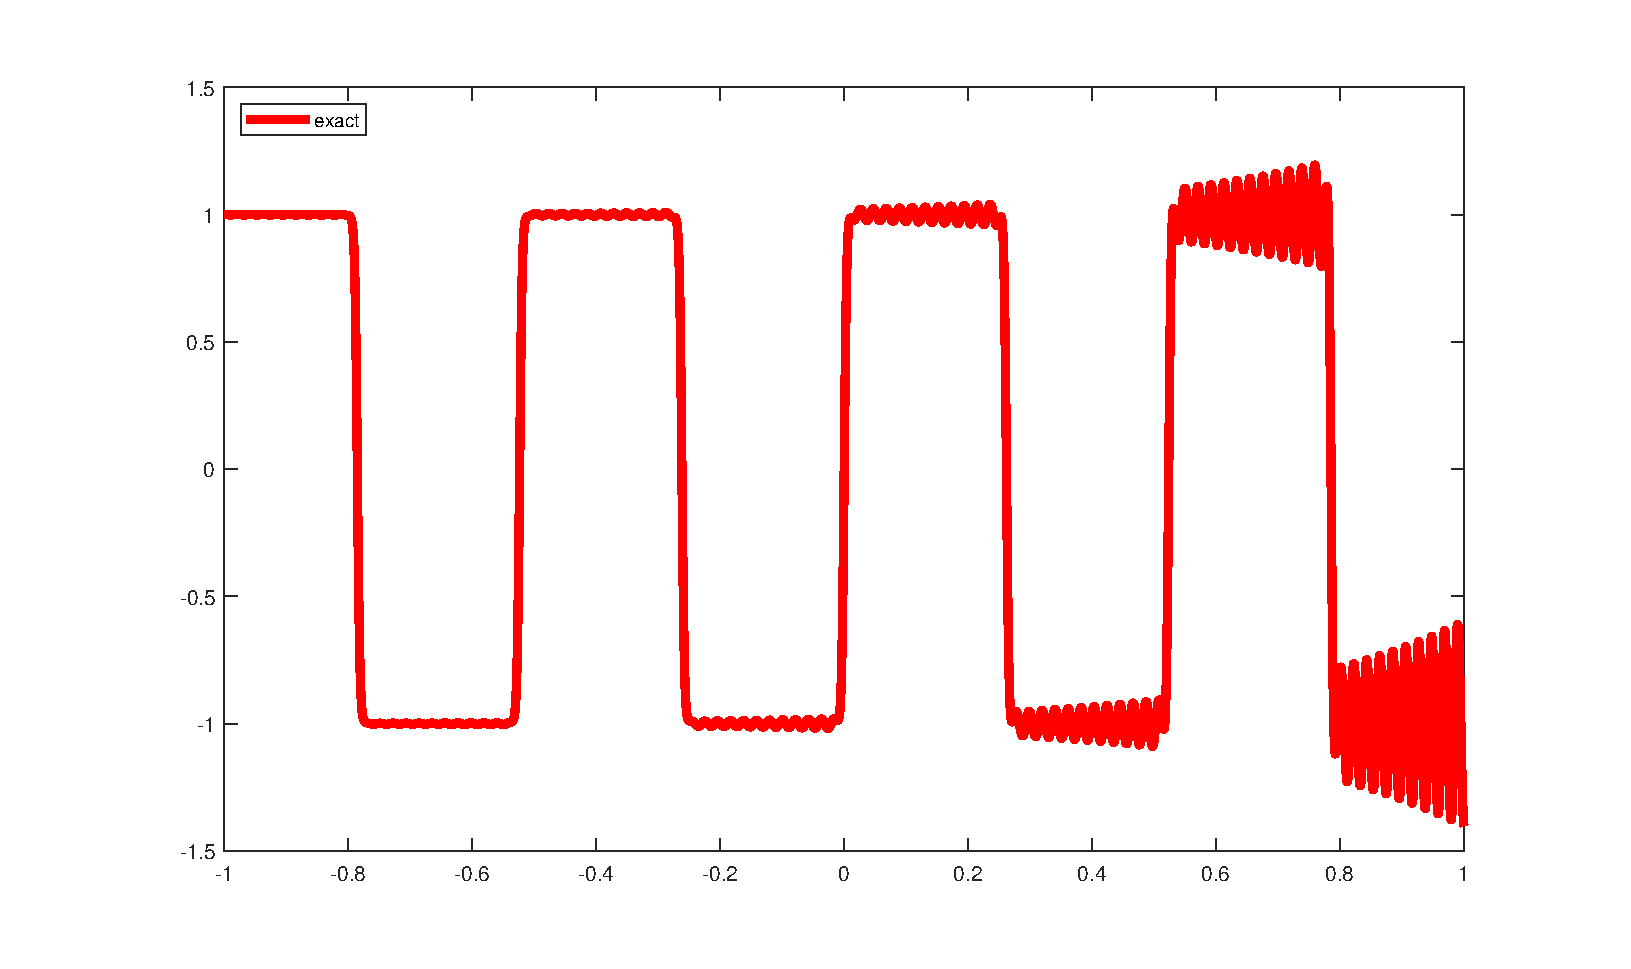
\includegraphics[width=1\textwidth]{p1d1.eps}
	\caption{(i)被插值函数}
\end{figure}

\begin{figure}[H]
	\centering
	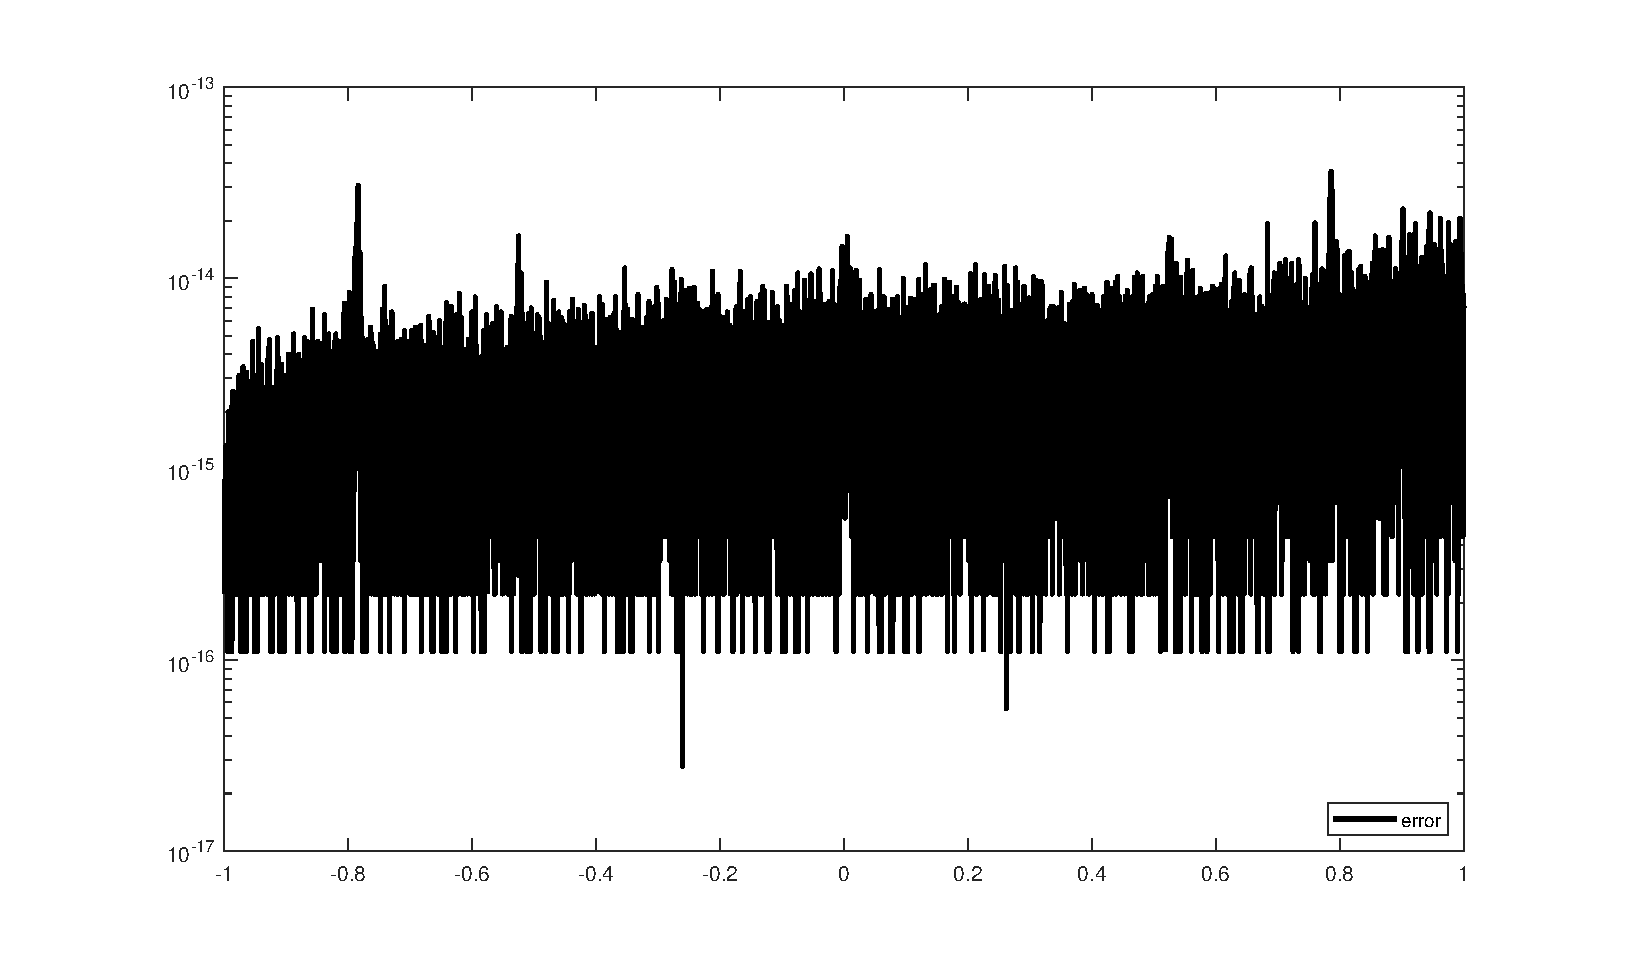
\includegraphics[width=1\textwidth]{p1d2.eps}
	\caption{(ii)误差}
\end{figure}

\item[第二题]

(a)
\textsc{Matlab}程序显示如下:
\begin{lstlisting}[frame=single]
clear, clc, clf
LW = 'linewidth'; lw = 2;
nn = zeros(7, 1);
maxq = zeros(7, 1);

for q = 6:12
      nn(q - 5) = 2^q;
      n = 2^q;
      x = linspace(-1, 1, n + 1)';
      F = @(x)exp (3 .* cos(pi .* x));
      f = F(x);
      h = diff(x);
      df = diff(f);
      lambda = h(2:n) ./ (h(2:n) + h(1:n - 1));
      d = 6 * (df(2:n) ./ h(2:n) - df(1:n - 1) ./ h(1:n - 1)) ./ (h(2:n) + h(1:n - 1));
      mu = 1 - lambda;
      
      %% 第一类边界条件
      M0 = 0;
      Mn = 0;
      A1 = diag(2 * ones(n - 1, 1)) + diag(lambda(1:n - 2), 1) + diag(mu(2:n - 1), -1);
      D1 = [d(1) - mu(1) * M0; d(2:n - 2); d(n - 1) - lambda(n - 1) * Mn];
      M1 = A1 \ D1;
      M1 = [M0; M1; Mn];
      %% 绘制图像
      figure(1);
      title('第一类边界条件样条插值效果');
      maxq(q - 5) = CubicSpline(x, F, h, M1, q); hold on
end

figure(2)
p3 = loglog(nn, maxq, 'b^-', 'MarkerFaceColor', 'b'); hold on
legend(p3, 'max error', 'location', 'se');
title('最大误差随n的log-log图');

function maxqq = CubicSpline(x, F, h, M, q)
LW = 'linewidth'; lw = 2;
n = size(x) - 1;
f = F(x);
areamax = zeros(2^q, 1);

for k = 1:n
      m = 4;
      xx = linspace(x(k), x(k + 1), m)';
      S = ((x(k + 1) - xx).^3 * M(k) + (xx - x(k)).^3 * M(k + 1)) / (6 * h(k)) + ...
         ((x(k + 1) - xx) * f(k) + (xx - x(k)) * f(k + 1)) / h(k) - ...
         h(k) * ((x(k + 1) - xx) * M(k) + (xx - x(k)) * M(k + 1)) / 6;
      
      p1 = plot(xx, F(xx), 'k', LW, lw); hold on
      p2 = plot(xx, S, 'r', LW, lw); hold on
      legend([p1, p2], 'exact', 'interpolant');
      error = abs(F(xx) - S);
      areamax(k) = max(error);
end

maxqq = max(areamax);
end
\end{lstlisting}
上述程序输出的图像为:
\begin{figure}[H]
	\centering
	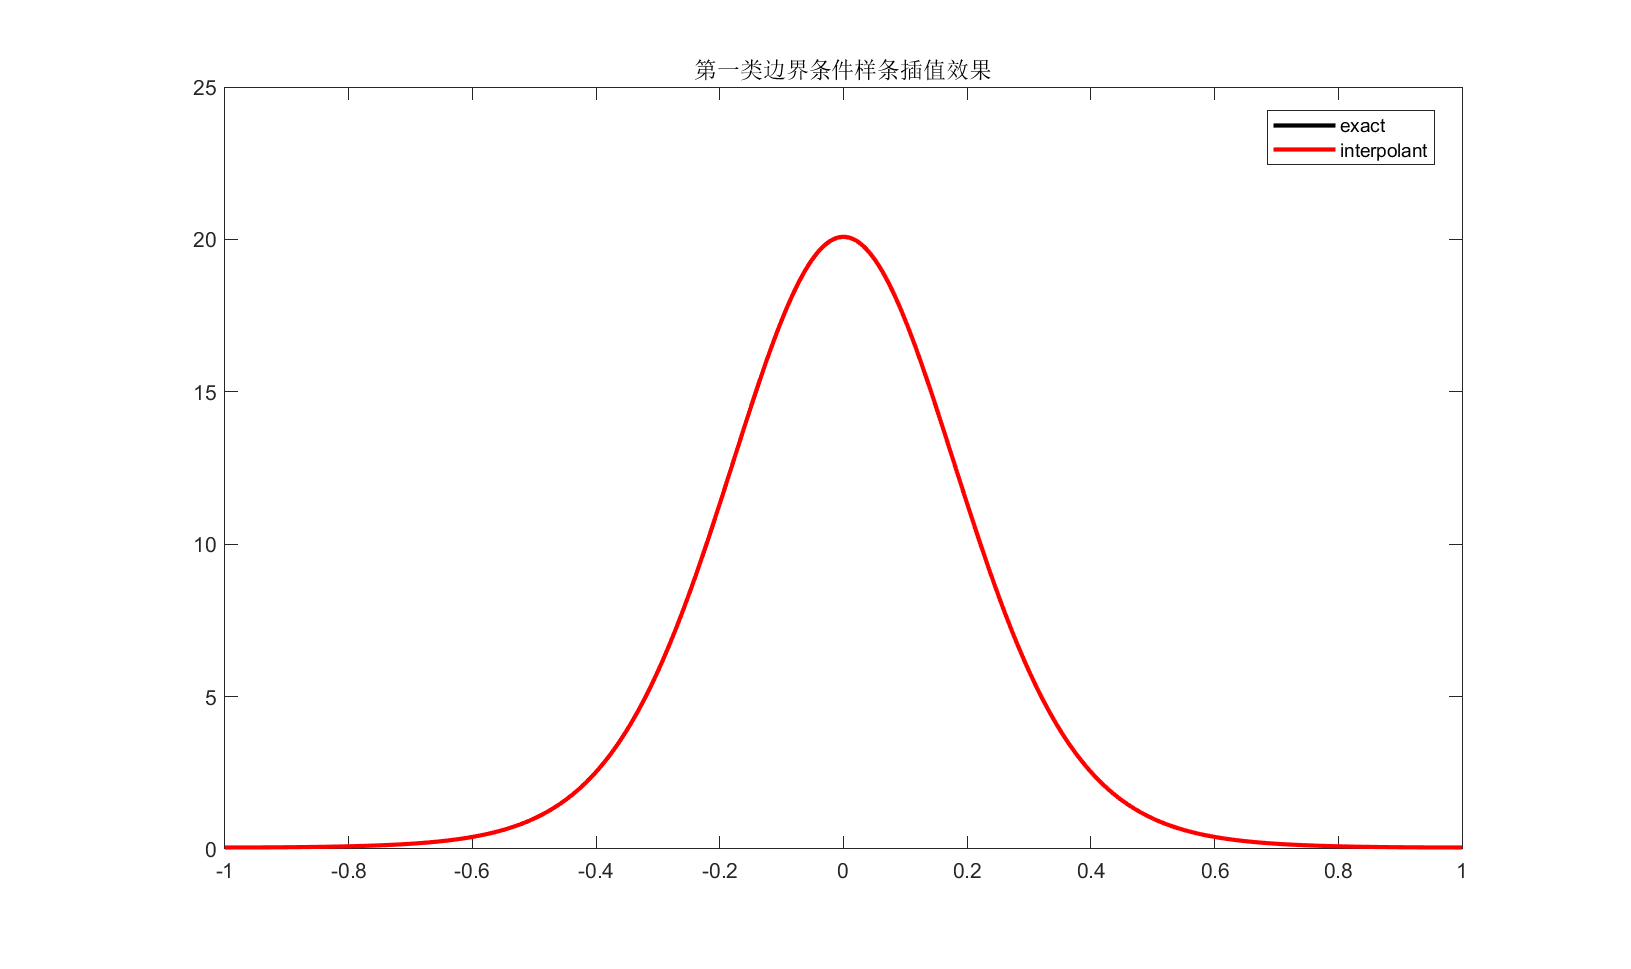
\includegraphics[width=1\textwidth]{p2a1.eps}
	\caption{第一类边界条件样条插值效果}
\end{figure}

\begin{figure}[H]
	\centering
	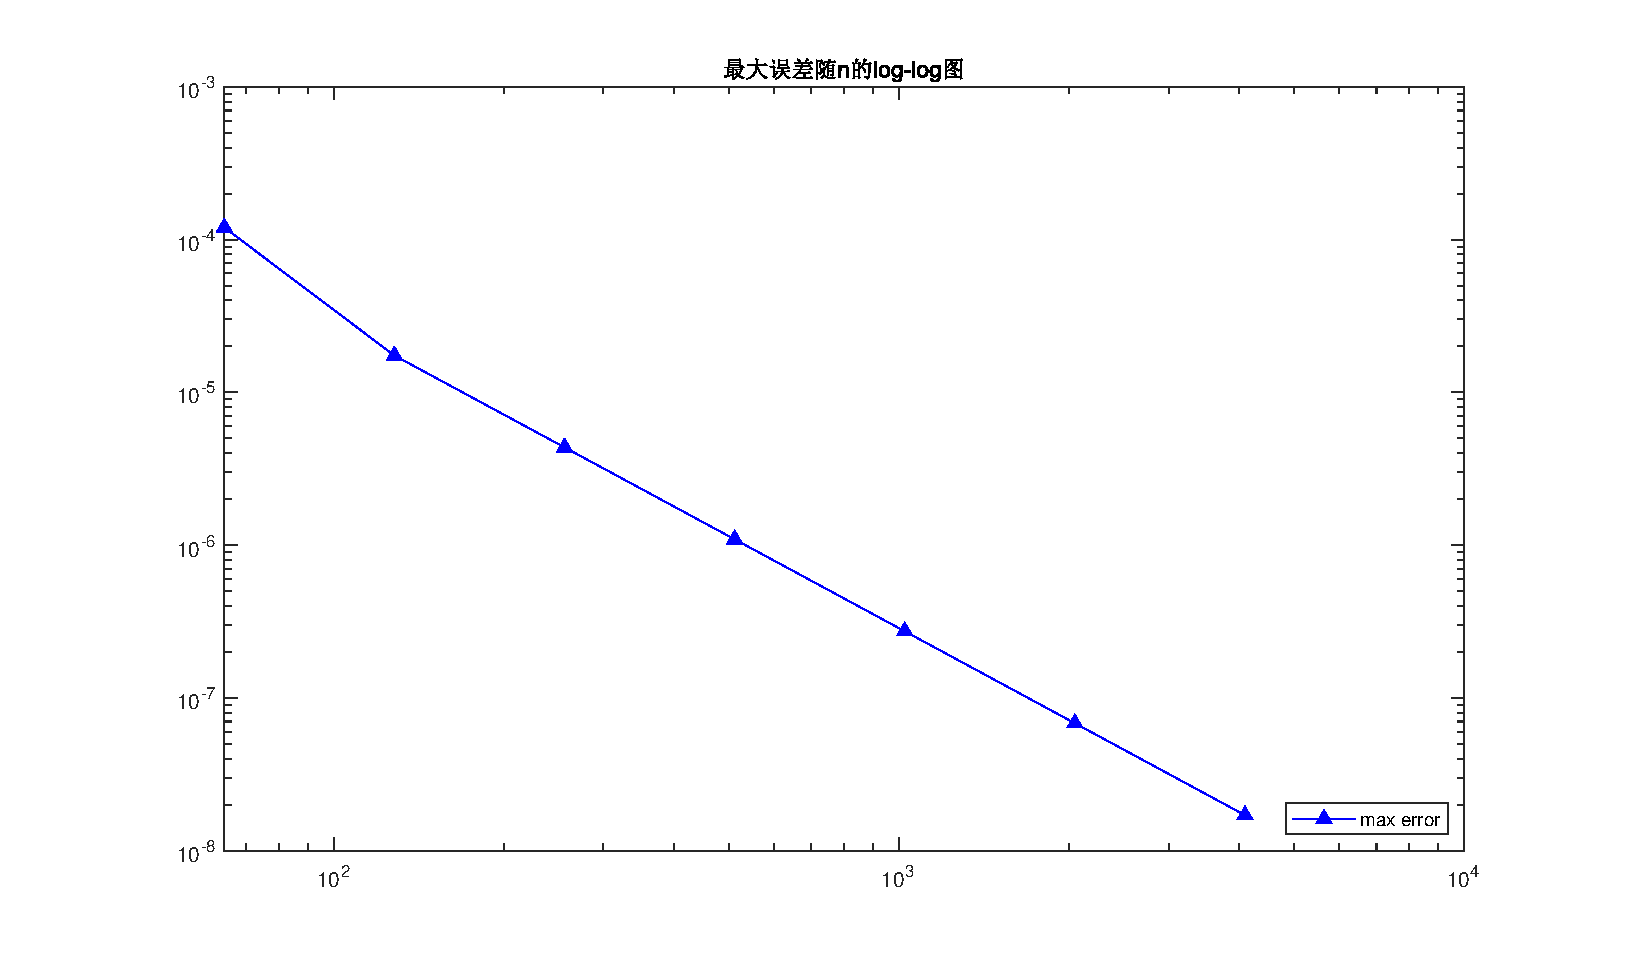
\includegraphics[width=1\textwidth]{p2a2.eps}
	\caption{最大误差随n的log-log图}
\end{figure}
(c)
\textsc{Matlab}程序显示如下:
\begin{lstlisting}[frame=single]
clear, clc, clf
LW = 'linewidth'; lw = 2;

nn = zeros(7, 1);
maxq1 = zeros(7, 1);
maxq2 = zeros(7, 1);
maxq3 = zeros(7, 1);

for q = 6:12
      nn(q - 5) = 2^q;
      n = 2^q;
      x = linspace(-1, 1, n + 1)';
      F = @(x)exp (3 .* cos(pi .* x));
      f = F(x);
      h = diff(x);
      df = diff(f);
      lambda = h(2:n) ./ (h(2:n) + h(1:n - 1));
      d = 6 * (df(2:n) ./ h(2:n) - df(1:n - 1) ./ h(1:n - 1)) ./ (h(2:n) + h(1:n - 1));
      mu = 1 - lambda;
      
      %% 第一类边界条件
      M0 = 0;
      Mn = 0;
      A1 = diag(2 * ones(n - 1, 1)) + diag(lambda(1:n - 2), 1) + diag(mu(2:n - 1), -1);
      D1 = [d(1) - mu(1) * M0; d(2:n - 2); d(n - 1) - lambda(n - 1) * Mn];
      M1 = A1 \ D1;
      M1 = [M0; M1; Mn];
      %% 第二类边界条件
      m0 = 0;
      mn = 0;
      lambda2 = [1; lambda];
      mu2 = [mu; 1];
      d0 = 6 * (df(1) / h(1) - m0) / h(1);
      dn = 6 * (mn - df(n) / h(n)) / h(n);
      D2 = [d0; d; dn];
      A2 = diag(2 * ones(n + 1, 1)) + diag(lambda2, 1) + diag(mu2, -1);
      M2 = A2 \ D2;
      %% 第三类边界条件
      lambda0 = h(1) / (h(1) + h(n));
      lambda3 = [lambda0; lambda(1:n - 2)];
      mu0 = 1 - lambda0;
      d0 = 6 * (df(1) ./ h(1) - df(n) ./ h(n)) / (h(1) + h(n));
      D3 = [d0; d];
      A3 = diag(2 * ones(n, 1)) + diag(lambda3, 1) + diag(mu, -1);
      A3(1, n) = mu0;
      A3(n, 1) = lambda(n - 1);
      M3 = A3 \ D3;
      M3 = [M3; M3(1)];
      %% 求最大误差
      maxq1(q - 5) = CubicSpline(x, F, h, M1, q);
      maxq2(q - 5) = CubicSpline(x, F, h, M2, q);
      maxq3(q - 5) = CubicSpline(x, F, h, M3, q);
end

%% 绘制图像
figure(1)
p3 = loglog(nn, maxq1, 'b^-', 'MarkerFaceColor', 'b'); hold on
p4 = loglog(nn, maxq2, 'ro-'); hold on
p5 = loglog(nn, maxq3, 'k*-', 'MarkerFaceColor', 'k'); hold on
legend([p3, p4, p5], '第一类边界条件', '第二类边界条件', '第三类边界条件')
title('三种边界条件下最大误差随n的log-log图')

function maxqq = CubicSpline(x, F, h, M, q)
n = size(x) - 1;
f = F(x);
areamax = zeros(2^q, 1);

for k = 1:n
      m = 4;
      xx = linspace(x(k), x(k + 1), m)';
      S = ((x(k + 1) - xx).^3 * M(k) + (xx - x(k)).^3 * M(k + 1)) / (6 * h(k)) + ...
         ((x(k + 1) - xx) * f(k) + (xx - x(k)) * f(k + 1)) / h(k) - ...
         h(k) * ((x(k + 1) - xx) * M(k) + (xx - x(k)) * M(k + 1)) / 6;
      error = abs(F(xx) - S);
      areamax(k) = max(error);
end

maxqq = max(areamax);
end
\end{lstlisting}
上述程序输出的图像为:
\begin{figure}[H]
	\centering
	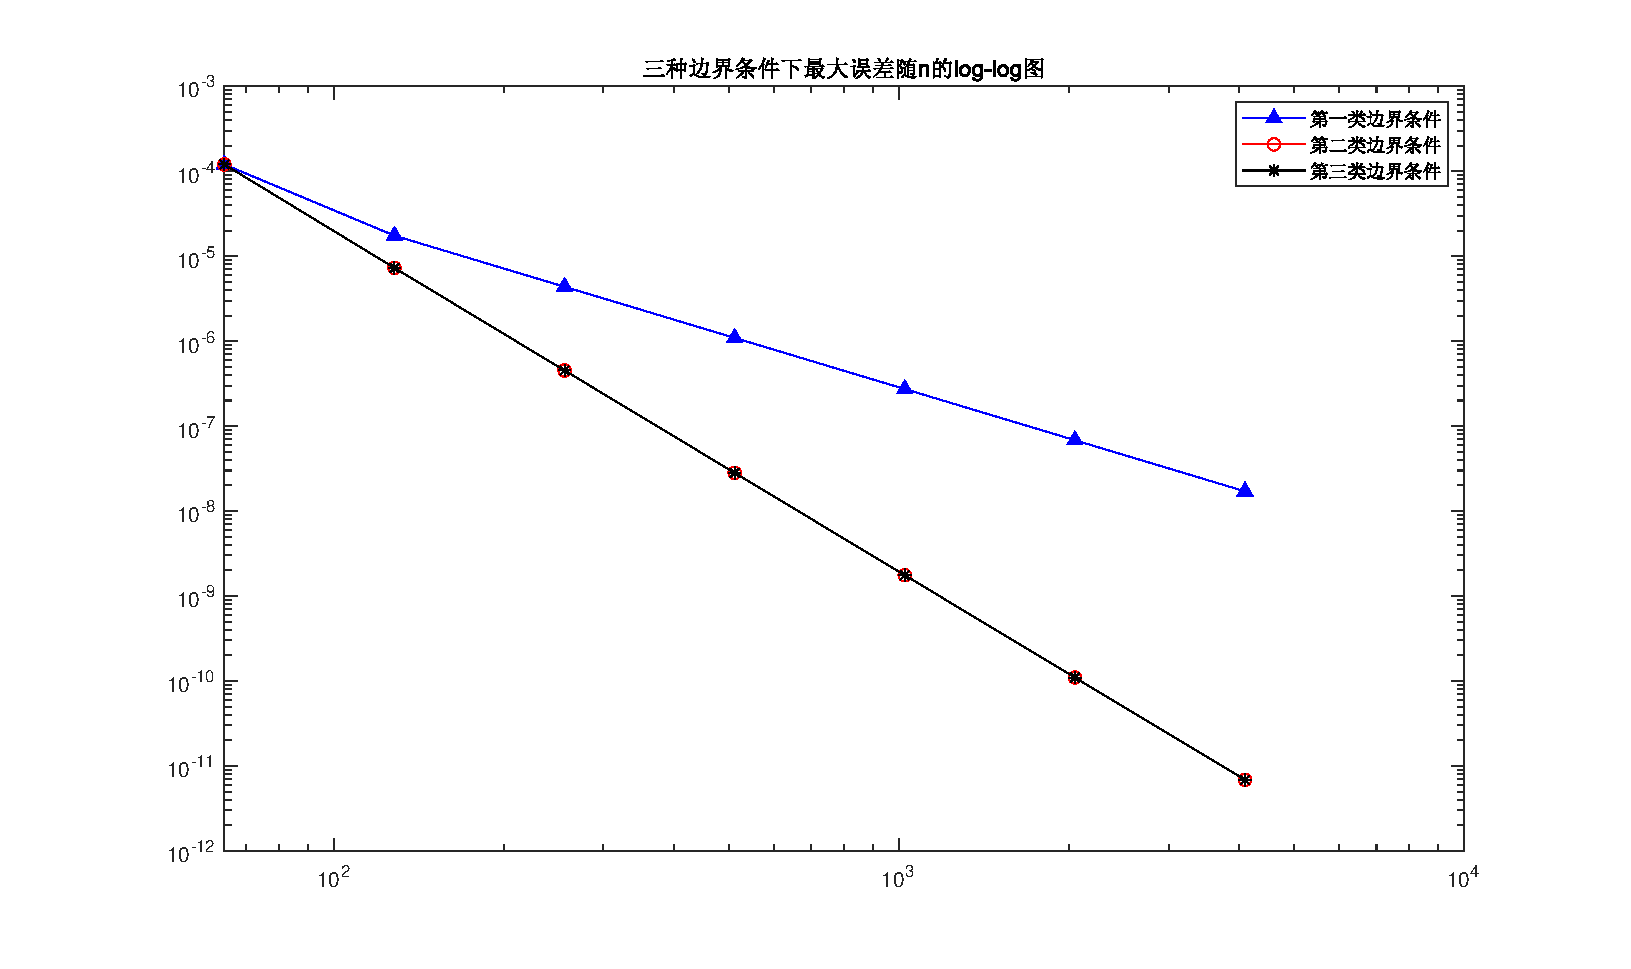
\includegraphics[width=1\textwidth]{p2c.eps}
	\caption{三种边界条件下最大误差随n的log-log图}
\end{figure}
\item[第三题]
\textsc{Matlab}程序显示如下:
\begin{lstlisting}[frame=single]
clear, clc, clf
LW = 'linewidth'; lw = 2;

x = [-0.7 -0.5 0.25 0.75];
y = [0.99 1.21 2.57 4.23];
y1 = log(y);
%%
% y1 = ln(y) = ln(a) + bx
% aa(1) = ln(a), aa(2) = b
M = zeros (2, 2);
bb = zeros (2, 1);
xx = linspace (-1, 1, 1000);
%% 线性拟合
M(1, 1) = 4;

for i = 1:4
      M(1, 2) = M(1, 2) + x(i);
      M(2, 1) = M(2, 1) + x(i);
      M(2, 2) = M(2, 2) + (x(i))^2;
      bb(1) = bb(1) + y1(i);
      bb(2) = bb(2) + x(i) * y1(i);
end

aa = M \ bb;
a = exp(aa(1));
b = aa (2);
F = @(x) a * exp(b * x);
figure(1)
p1 = plot(x, y, 'o', LW, lw); hold on
plot(xx, F(xx), LW, lw);
h = legend('$$y_i$$', sprintf('$$y=%fe^{%fx}$$', a, b));
set(h, 'Interpreter', 'latex', 'FontSize', 24, 'FontWeight', 'bold');
%% 计算拟合函数的误差的2-范数
format long
error = abs(F(x) - y);
norm2 = sqrt(sum(error .* error))
%% 输出 norm2 = 0.006154650408178
\end{lstlisting}
上述程序输出的图像为:
\begin{figure}[H]
	\centering
	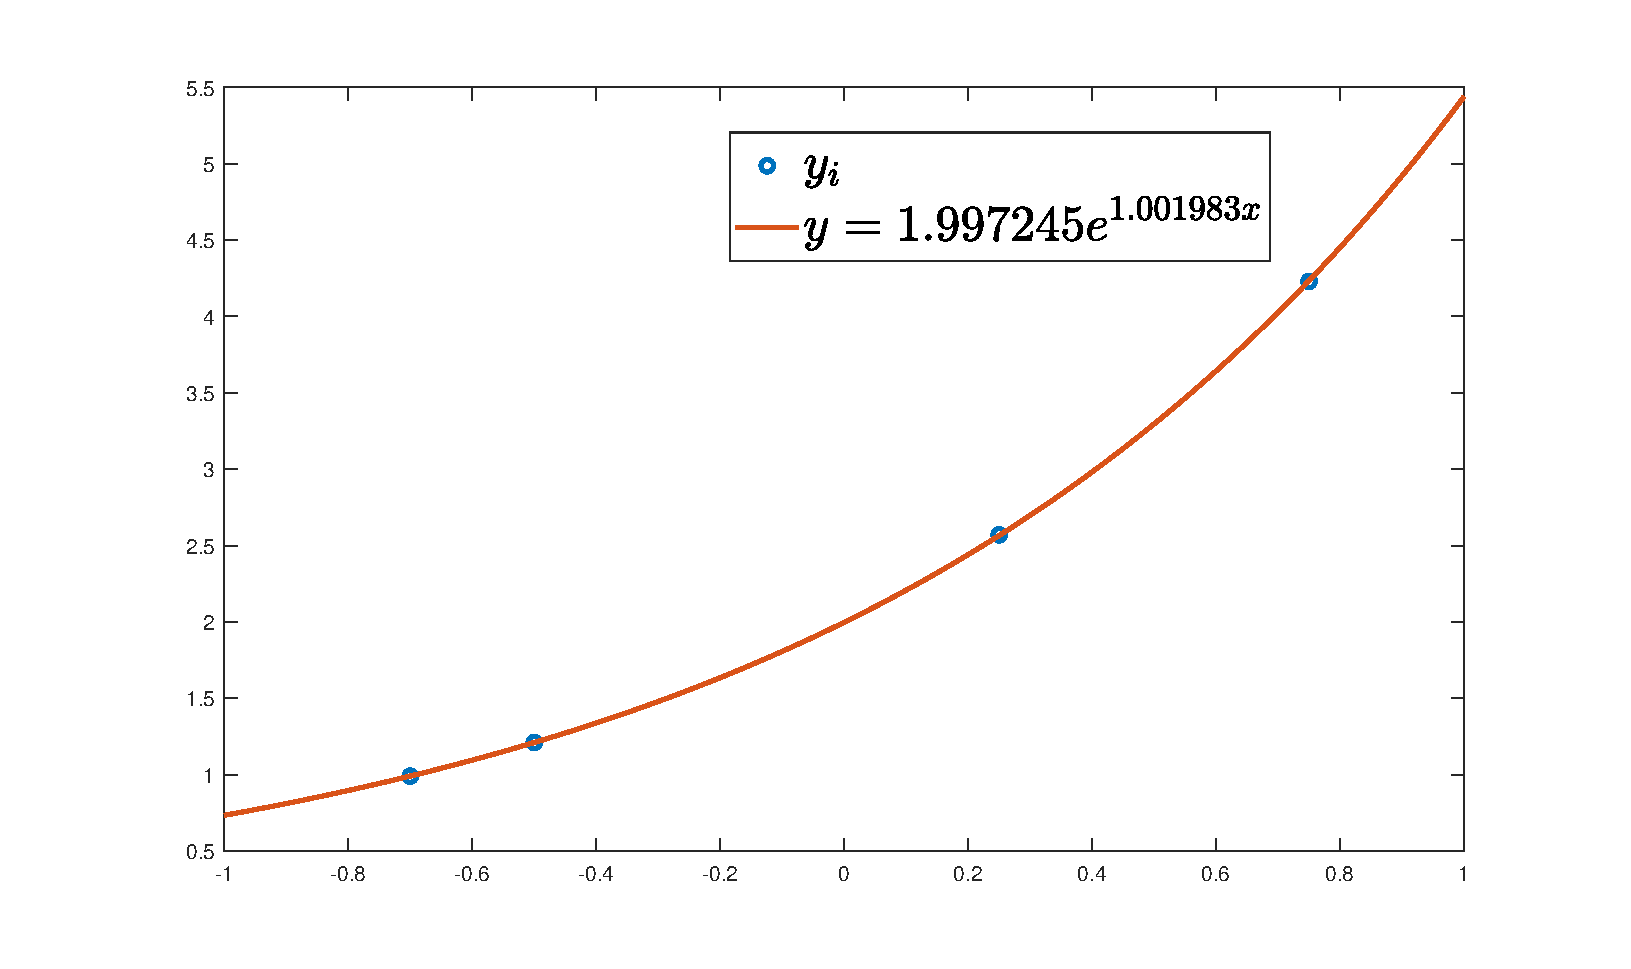
\includegraphics[width=1\textwidth]{p3.eps}
	\caption{数据和拟合函数}
\end{figure}
即拟合函数表达式为:
\begin{equation}
   y=1.997245e^{1.001983x} \nonumber
\end{equation}
命令行窗口输出拟合函数的误差的2-范数:$norm2 = 0.006154650408178$
\end{enumerate}
\end{document}
